\documentclass[11pt,a4paper]{ltjsarticle}

\usepackage{amsmath,amssymb}
\usepackage{booktabs}
\usepackage{longtable}
\usepackage{graphicx}
\usepackage{geometry}
\usepackage{hyperref}
\geometry{margin=25mm}
\hypersetup{colorlinks=true,linkcolor=blue,urlcolor=blue}

\title{Spectral-Parameter Learning for Lax Connections\\研究ノート}
\author{}
\date{2026年9月13日}

\begin{document}
\maketitle

\section{目的}

本ノートは，既発表論文
\begin{center}
O.~Fukushima, T.~Shigemura, R.~Suda, N.~Tanahashi and K.~Yoshida,
``Machine-Learning Search for Lax Connections,''
\href{https://arxiv.org/abs/2608.05146}{arXiv:2608.05146}
\end{center}
の後続研究として，スペクトルパラメータを含む Lax connection の機械学習を整理するための作業ノートである．共同研究者から共有された二つの計算ノートに含まれる取り組みを整理し，既発表論文に含まれる内容と未発表の差分を区別する．その後，追加の数値検証を順次記録する．

本ノートでは，各節を単独で読んでも計算設定を復元できることを優先する．研究グループ内だけで通用する分類名を前提にせず，場，current，微分方程式，residual，学習対象，損失関数，評価量を初出時に定義する．略語は原則として用いない．

\section{共同研究者ノートに含まれる取り組み}

比較対象は次の二つである．
\begin{enumerate}
  \item N.~Tanahashi, ``Explicit Spectral-Parameter Learning in the PCM: Implementation Notes and Numerical Results,'' May 24, 2026.
  \item N.~Tanahashi, ``Machine-Learning the Spectral Parameter for the $S^2$ Coset: Prior-Free Discovery, Tracing, and Charting of the Lax Family,'' June 9, 2026.
\end{enumerate}

第一のノートは $SU(2)$ principal chiral model に対して三種類の損失構成を比較している．第二のノートは $S^2=SU(2)/U(1)$ sigma model に対して，flatness solution set の局所構造の同定，continuation による追跡，複素スペクトルパラメータを入力する neural network による表現，の三段階を扱っている．この区分に従うと，主要な取り組みは合計六項目である．

\subsection{Principal chiral model: bare flatness loss と再パラメータ化自由度}

current を $J_\pm$ とし，
\begin{equation}
L_+=a(\lambda)J_+,
\qquad
L_-=c(\lambda)J_-
\end{equation}
という Lax connection の ansatz を用いる．複素スペクトルパラメータ $\lambda$ に依存する追加の重みを用いず，flatness residual の二乗を損失関数とする基準計算である．

同時に，$a(\lambda)$ と $c(\lambda)$ をともに学習する場合，$a(\lambda)$ を既知関数として固定する場合，$a(\lambda)$ を既知関数の近傍に penalty で拘束する場合を比較する．flatness が係数間の代数関係だけを決め，スペクトルパラメータの取り方には再パラメータ化自由度が残ることを調べる．

\subsection{Principal chiral model: analytic per-$\lambda$ reweighting}

$a(\lambda)=\lambda$ を固定した場合に，flatness loss から $c(\lambda)$ に伝わる勾配強度の $\lambda$ 依存性を解析し，
\begin{equation}
w(\lambda)\propto\left|\lambda-\frac12\right|^{-2}
\end{equation}
という解析的な重みを導入する．目的は，スペクトルパラメータ領域内で不均一な training signal を補償することである．

\subsection{Principal chiral model: component-norm normalization と adaptive $\lambda$ weighting}

解析解や principal chiral model 固有の勾配公式を使わずに training signal の不均一性を抑える．flatness residual を構成する各項の norm を用いる component-norm normalization と，学習中に測定した各 $\lambda$ における loss の exponential moving average に基づく adaptive weighting を組み合わせる．

\subsection{$S^2=SU(2)/U(1)$ sigma model: Jacobian の null space から family を同定する計算}

Lie algebra current を $\mathfrak h\oplus\mathfrak m$ に分解し，
\begin{equation}
J_\pm=J_\pm^{(0)}+J_\pm^{(1)}
\end{equation}
とする．Lax connection の線形 ansatz を
\begin{equation}
L_+=aJ_+^{(0)}+bJ_+^{(1)},
\qquad
L_-=cJ_-^{(0)}+dJ_-^{(1)}
\end{equation}
と置く．flatness residual を係数 $(a,b,c,d)$ の関数とみなし，その Jacobian の null space を調べる．nullity から flatness solution set の局所次元を推定し，null vector の成分から変化しない係数と family に沿って変化する係数を識別する．さらに，null-vector field と収束点の集合から保存される係数の組合せを抽出し，$a=c=1$ と $bd=1$ を事前に仮定せずに再構成する．

\subsection{$S^2=SU(2)/U(1)$ sigma model: pseudo-arclength continuation}

Jacobian の null space で得られた局所 tangent direction を用いて predictor--corrector 型の pseudo-arclength continuation を行い，flatness solution manifold 上の連続な経路を追跡する．一複素次元の solution manifold は二実次元なので，この計算が追うのは manifold 全体ではなく，その内部の一実次元の path である．

\subsection{$S^2=SU(2)/U(1)$ sigma model: 複素スペクトルパラメータを入力とする neural network}

複素スペクトルパラメータを入力とする neural network
\begin{equation}
\mathcal N:\lambda\in\mathbb C\longmapsto
(a(\lambda),b(\lambda),c(\lambda),d(\lambda))\in\mathbb C^4
\end{equation}
を学習し，flatness solution manifold の有限領域を滑らかで微分可能な map として表現する．学習には component-norm normalized flatness loss に加え，$\lambda$ に依存しない map への collapse を防ぐ derivative term と，continuation で得た solution points を用いる anchor term を用いる．

\section{既発表論文との差分}

既発表論文では，principal chiral model について $a(\lambda)=\lambda$ を固定して $c(\lambda)$ を neural network で学習する計算と component-norm normalized flatness loss がすでに含まれている．また $S^2=SU(2)/U(1)$ sigma model については，$a,b,c,d$ の定数学習に加え，truncated Laurent ansatz によって明示的な $\lambda$ dependence を学習している．したがって，「スペクトルパラメータを明示的に扱うこと」だけでは新しい差分にならない．

\begin{longtable}{p{0.06\textwidth}p{0.29\textwidth}p{0.38\textwidth}p{0.17\textwidth}}
\toprule
No. & 共同研究者ノートの項目 & 既発表論文との関係 & 位置づけ \\
\midrule
1 & Principal chiral model: bare flatness loss と三種類の $a(\lambda)$ の扱い
& 既発表論文は $a(\lambda)$ の固定と component-norm normalization を用いる．bare loss を含む系統比較は未掲載．
& 基準計算と ablation \\
\addlinespace
2 & Principal chiral model: analytic per-$\lambda$ reweighting
& $\lambda$ による勾配不均一性から解析的な重みを導く比較は未掲載．
& 明確な方法論的差分 \\
\addlinespace
3 & Principal chiral model: component-norm normalization と adaptive weighting
& component-norm normalization 自体は既発表論文に含まれるが，学習中の loss に基づく adaptive weighting と他手法との比較は未掲載．
& 部分的な方法論的差分 \\
\addlinespace
4 & $S^2$: Jacobian null-space analysis
& 既発表論文は収束点の集合と Laurent ansatz から family を確認するが，Jacobian の nullity と null vectors から family dimension と invariant を抽出する手順は含まない．
& 明確な方法論的差分 \\
\addlinespace
5 & $S^2$: pseudo-arclength continuation
& solution manifold を tangent direction に沿って continuation する計算は未掲載．
& 明確な方法論的差分 \\
\addlinespace
6 & $S^2$: neural-network chart
& 既発表論文の明示的な $\lambda$ dependence は truncated Laurent ansatz であり，continuation points を anchor とする neural-network chart は未掲載．
& 明確な方法論的差分 \\
\bottomrule
\end{longtable}

共同研究者ノートの六項目すべてに，少なくとも未発表の比較または数値結果が含まれる．新しい方法として数えると，五項目が未発表の method element を含み，そのうち四項目は既発表論文から明確に切り分けられる．

\section{追加検証1：principal chiral model における off-shell factorization}

共同研究者ノートとは別に，Lax curvature が equation of motion をどの程度 encode しているかを直接調べる．この検証では，flatness を満たす on-shell data だけを使うのではなく，Maurer--Cartan identity は満たすが equation of motion は満たさない data を用いる．

\subsection{物理的設定}

$SU(2)$ principal chiral model の群値場を $g(x)$ とし，light-cone coordinates における right-invariant current を
\begin{equation}
J_\pm:=g^{-1}\partial_\pm g
\end{equation}
と定義する．この current は Maurer--Cartan identity
\begin{equation}
\partial_+J_- - \partial_-J_+ +[J_+,J_-]=0
\label{eq:mc-pcm}
\end{equation}
を恒等的に満たす．一方，equation of motion は
\begin{equation}
\partial_+J_-+\partial_-J_+=0
\end{equation}
である．equation-of-motion residual を
\begin{equation}
E:=\partial_+J_-+\partial_-J_+
\label{eq:eom-residual-pcm}
\end{equation}
と定義する．

標準的な Lax connection を
\begin{equation}
L_+(\lambda)=\frac{1}{1-\lambda}J_+,
\qquad
L_-(\lambda)=\frac{1}{1+\lambda}J_-
\label{eq:pcm-lax}
\end{equation}
とする．Lax curvature を
\begin{equation}
F_{+-}(\lambda)
:=\partial_+L_-(\lambda)-\partial_-L_+(\lambda)
+[L_+(\lambda),L_-(\lambda)]
\end{equation}
と定義する．式~\eqref{eq:mc-pcm} を使うと，equation of motion を課す前に
\begin{equation}
F_{+-}(\lambda)=Q(\lambda)E,
\qquad
Q(\lambda)=-\frac{\lambda}{1-\lambda^2}\,\mathbf 1_{\mathfrak{su}(2)}
\label{eq:pcm-exact-q}
\end{equation}
と因数分解できる．$\mathbf 1_{\mathfrak{su}(2)}$ は三次元 Lie algebra $\mathfrak{su}(2)$ 上の恒等写像である．

\subsection{学習 data と neural network}

解析式~\eqref{eq:pcm-exact-q} は学習器に与えない．Lie algebra basis を $T_a$ $(a=1,2,3)$ とし，$E=E^aT_a$ と $F_{+-}=F^aT_a$ の成分を用いる．neural network は
\begin{equation}
(\operatorname{Re}\lambda,\operatorname{Im}\lambda)\in\mathbb R^2
\end{equation}
を入力とし，一般の複素 $3\times3$ matrix $Q^a{}_b(\lambda)$ を出力する．対角 matrix であること，三つの対角成分が等しいこと，有理関数であることは architecture に与えない．

各 training sample では $J_+$，$J_-$，$E$ を独立に乱数生成する．$C:=[J_+,J_-]$ と定義して
\begin{equation}
\partial_+J_-:=\frac{E-C}{2},
\qquad
\partial_-J_+:=\frac{E+C}{2}
\label{eq:pcm-offshell-sampling}
\end{equation}
と置く．これにより Maurer--Cartan identity は sample ごとに正確に満たされるが，$E$ は一般にゼロではない．

損失関数は
\begin{equation}
\mathcal L_Q
=
\frac{\left\langle\lVert F_{+-}(\lambda)-Q(\lambda)E\rVert^2\right\rangle}
{\left\langle\lVert F_{+-}(\lambda)\rVert^2\right\rangle+10^{-30}}
\label{eq:pcm-q-loss}
\end{equation}
とした．training domain は
\begin{equation}
-0.75\leq\operatorname{Re}\lambda\leq0.75,
\qquad
-0.75\leq\operatorname{Im}\lambda\leq0.75
\end{equation}
である．neural network は三 hidden layers，各 128 units，tanh activation を用いる．学習は 4000 steps，batch size 4096，Adam optimizer，learning rate $2\times10^{-3}$ で行った．

\subsection{一回の学習結果}

random seed 1234 の一回目の計算では，held-out data に対して
\begin{equation}
\frac{\lVert F_{+-}-QE\rVert}{\lVert F_{+-}\rVert}
=2.83\times10^{-2}
\end{equation}
であった．解析解との相対 matrix error も $2.83\times10^{-2}$ であった．学習された matrix 全体の Frobenius norm に対する off-diagonal entries の norm の割合は $7.49\times10^{-3}$，三つの diagonal entries の相対 spread は $4.89\times10^{-3}$ である．一般の複素 $3\times3$ matrix を出力させても，学習結果は scalar multiple of the identity に近づいた．

\begin{figure}[tb]
  \centering
  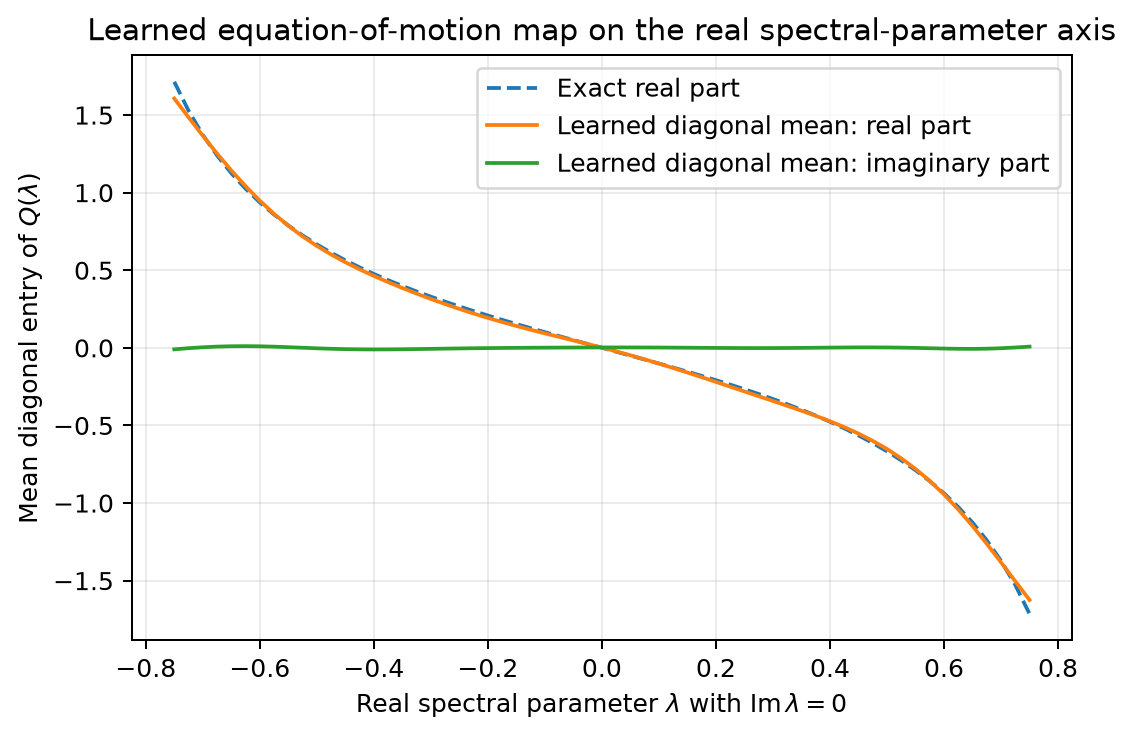
\includegraphics[width=0.80\linewidth]{../figures/01_pcm_fqe/q_diagonal_real_axis.png}
  \caption{$\operatorname{Im}\lambda=0$ における学習された $Q(\lambda)$ の diagonal entries の平均と，学習に使用していない解析解の比較．}
  \label{fig:pcm-q-single-diagonal}
\end{figure}

複素スペクトルパラメータ領域の pointwise error は domain の内部より境界付近で大きい．

\begin{figure}[tb]
  \centering
  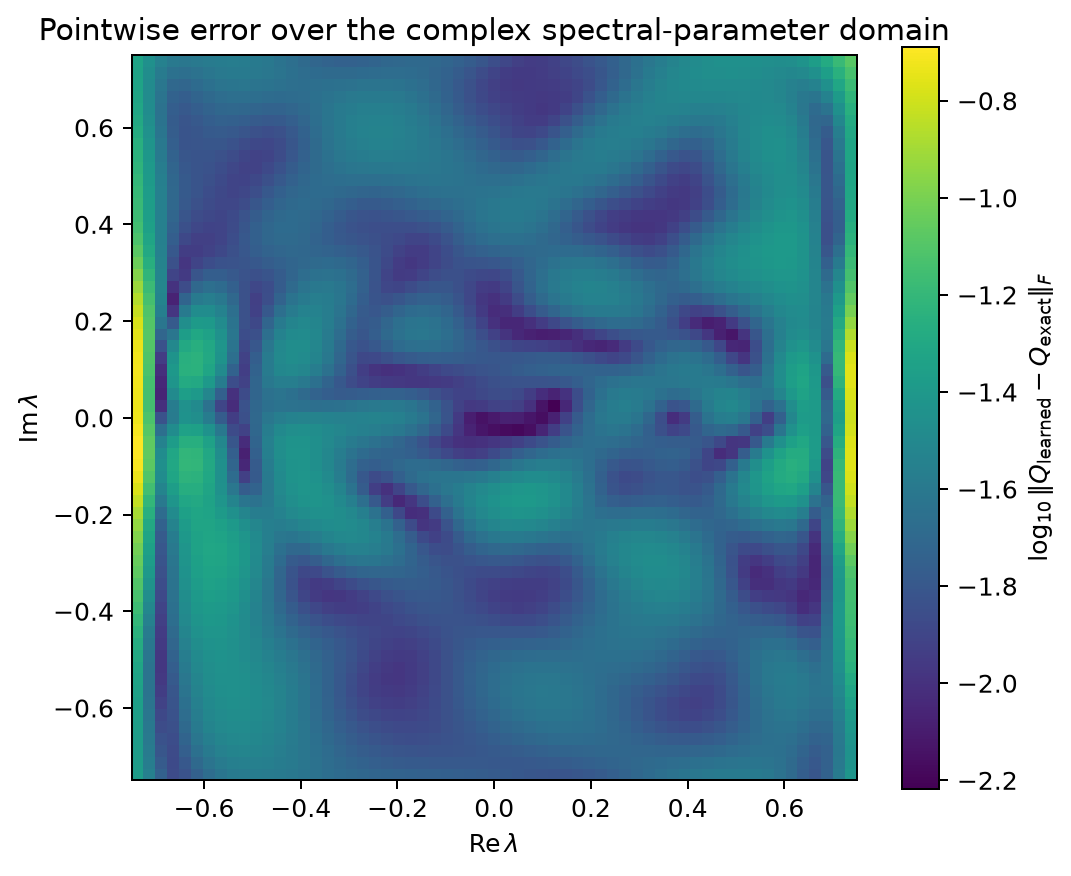
\includegraphics[width=0.76\linewidth]{../figures/01_pcm_fqe/q_error_complex_plane.png}
  \caption{複素スペクトルパラメータ領域における pointwise Frobenius error．}
  \label{fig:pcm-q-single-plane}
\end{figure}

\subsection{五つの独立な初期値を用いた再現性確認}

一回の neural-network optimization に依存した結果でないことを確認するため，random seed
\begin{equation}
1234,\quad 2026,\quad 2718,\quad 4242,\quad 31415
\end{equation}
を用いて，network architecture，training domain，batch size，学習率，training steps を同一に保った五回の独立な学習を行った．結果を表~\ref{tab:pcm-q-multiseed} にまとめる．standard deviation は五回の sample standard deviation である．

\begin{table}[tb]
\centering
\begin{tabular}{lcc}
\toprule
評価量 & 平均 & standard deviation \\
\midrule
$\lVert F_{+-}-QE\rVert/\lVert F_{+-}\rVert$
& $2.96\times10^{-2}$ & $5.57\times10^{-3}$ \\
$\lVert Q_{\rm learned}-Q_{\rm exact}\rVert_F/\lVert Q_{\rm exact}\rVert_F$
& $2.97\times10^{-2}$ & $5.59\times10^{-3}$ \\
off-diagonal norm fraction
& $1.25\times10^{-2}$ & $6.20\times10^{-3}$ \\
diagonal-entry relative spread
& $4.37\times10^{-3}$ & $6.80\times10^{-4}$ \\
\bottomrule
\end{tabular}
\caption{五つの random seed に対する独立な学習結果．解析解は学習 loss には用いていない．}
\label{tab:pcm-q-multiseed}
\end{table}

held-out residual は $2.10\times10^{-2}$ から $3.45\times10^{-2}$ の範囲，解析解との相対 matrix error は $2.10\times10^{-2}$ から $3.46\times10^{-2}$ の範囲に入った．したがって，約三パーセントの関数近似精度は特定の初期値だけで生じたものではない．diagonal-entry relative spread は全 run で $5.4\times10^{-3}$ 未満であり，三つの diagonal entries が同じ関数へ近づく構造は特に安定している．off-diagonal norm fraction は $6.48\times10^{-3}$ から $2.23\times10^{-2}$ と変動が大きいが，全 run で数パーセント以下である．

\begin{figure}[tb]
  \centering
  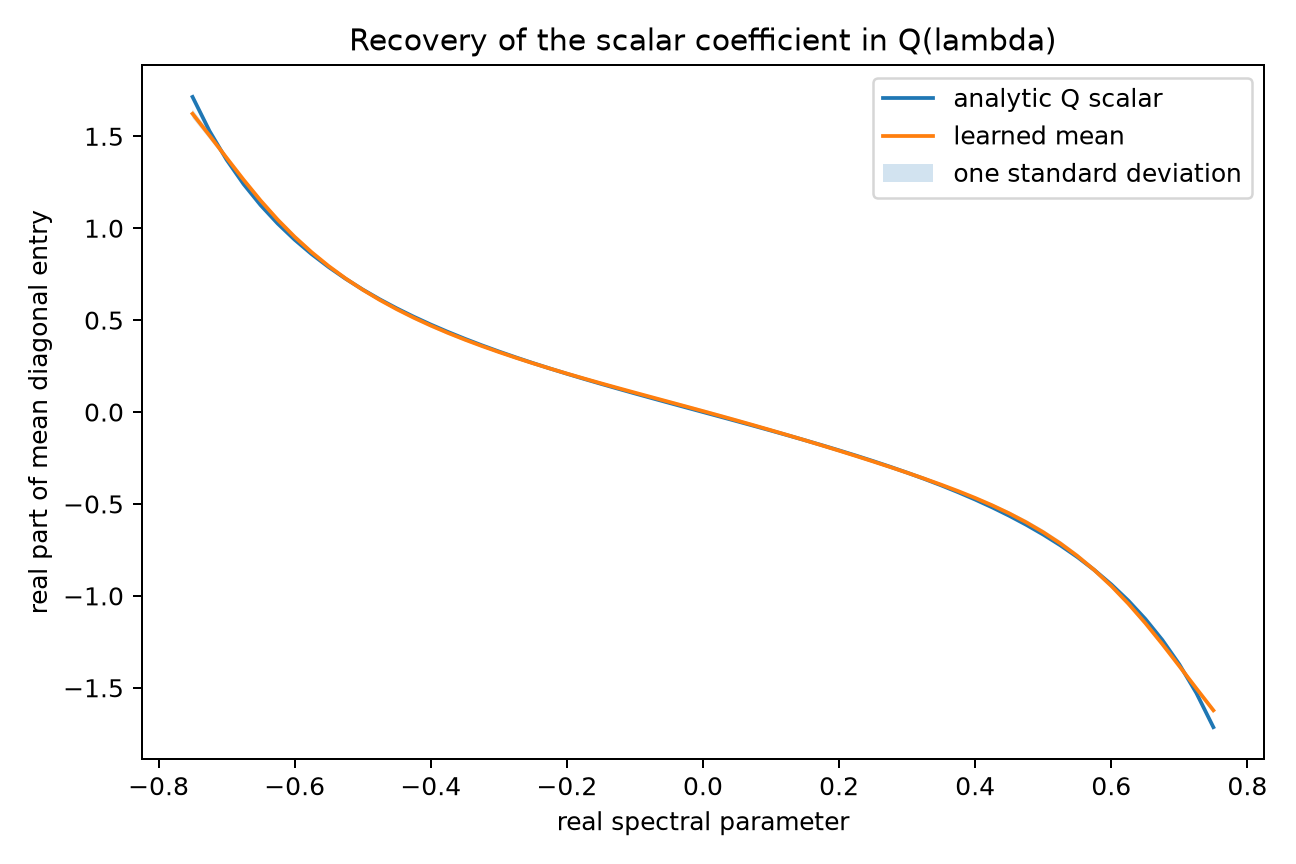
\includegraphics[width=0.82\linewidth]{../figures/01_pcm_fqe_multiseed/q_diagonal_real_axis_multiseed.png}
  \caption{五つの独立な学習で得た $Q(\lambda)$ の diagonal entries の平均．帯は run 間の一 standard deviation を表す．}
  \label{fig:pcm-q-multiseed-diagonal}
\end{figure}

図~\ref{fig:pcm-q-multiseed-plane} は，各複素スペクトルパラメータにおける Frobenius error を五回の run で平均したものである．単一 run と同様，domain boundary 付近で誤差が増える傾向が再現された．したがって，この特徴は一つの initialization に固有ではなく，現在の一様 sampling と finite network approximation に共通する系統的な誤差である可能性が高い．

\begin{figure}[tb]
  \centering
  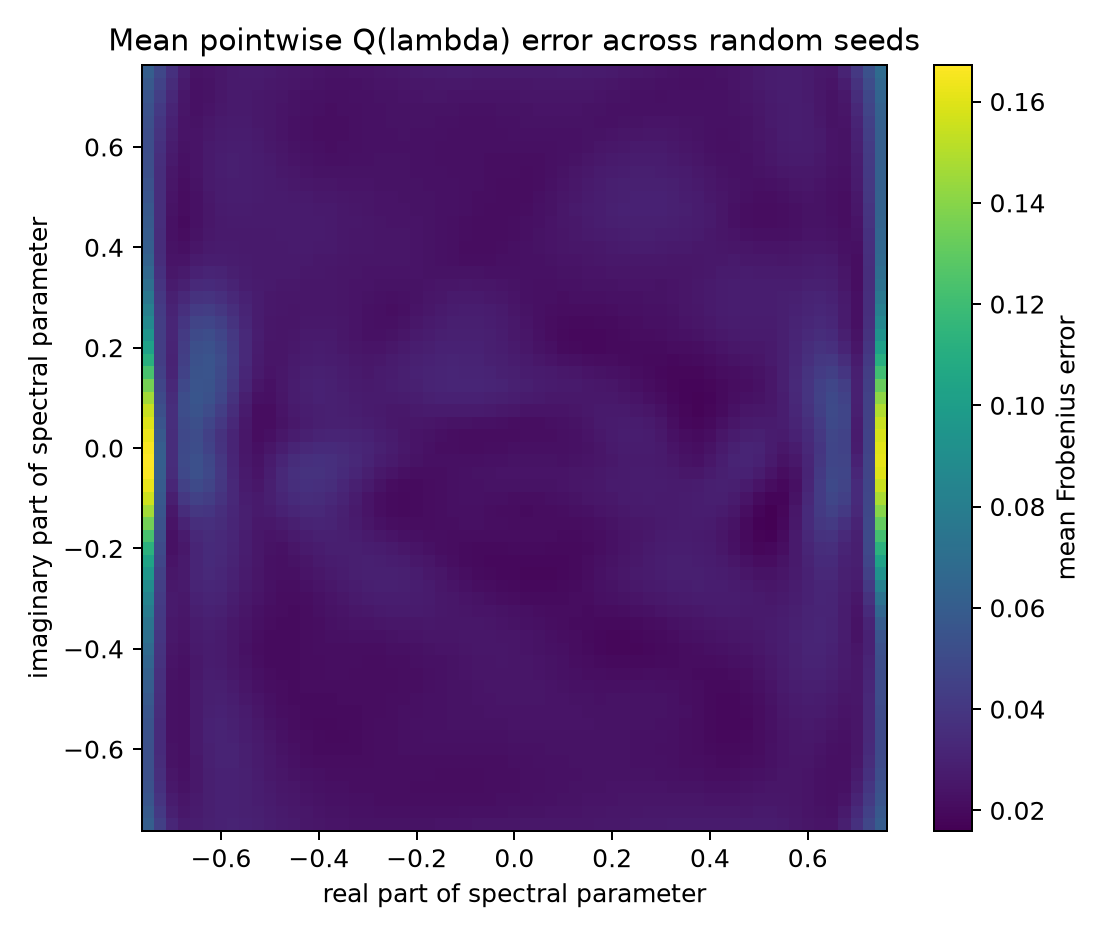
\includegraphics[width=0.76\linewidth]{../figures/01_pcm_fqe_multiseed/q_error_complex_plane_multiseed_mean.png}
  \caption{複素スペクトルパラメータ領域における pointwise Frobenius error の五 run 平均．}
  \label{fig:pcm-q-multiseed-plane}
\end{figure}

\subsection{$\lambda=0$ における singular values と rank の扱い}

解析式~\eqref{eq:pcm-exact-q} から，$\lambda\neq0,\pm1$ では $Q(\lambda)$ は三つの Lie algebra directions に対して full rank である．一方，$\lambda=0$ では
\begin{equation}
L_+(0)=J_+,
\qquad
L_-(0)=J_-,
\qquad
Q(0)=0
\end{equation}
となる．この点では flatness は equation of motion ではなく Maurer--Cartan identity だけから成立する．

五つの独立な学習における $\lambda=0$ での learned $Q$ の operator norm は平均 $1.63\times10^{-2}$，standard deviation $5.12\times10^{-3}$ であった．三 singular values の run 平均は
\begin{equation}
1.63\times10^{-2},\qquad
1.16\times10^{-2},\qquad
8.90\times10^{-3}
\end{equation}
であり，解析的にはすべてゼロである．

\begin{figure}[tb]
  \centering
  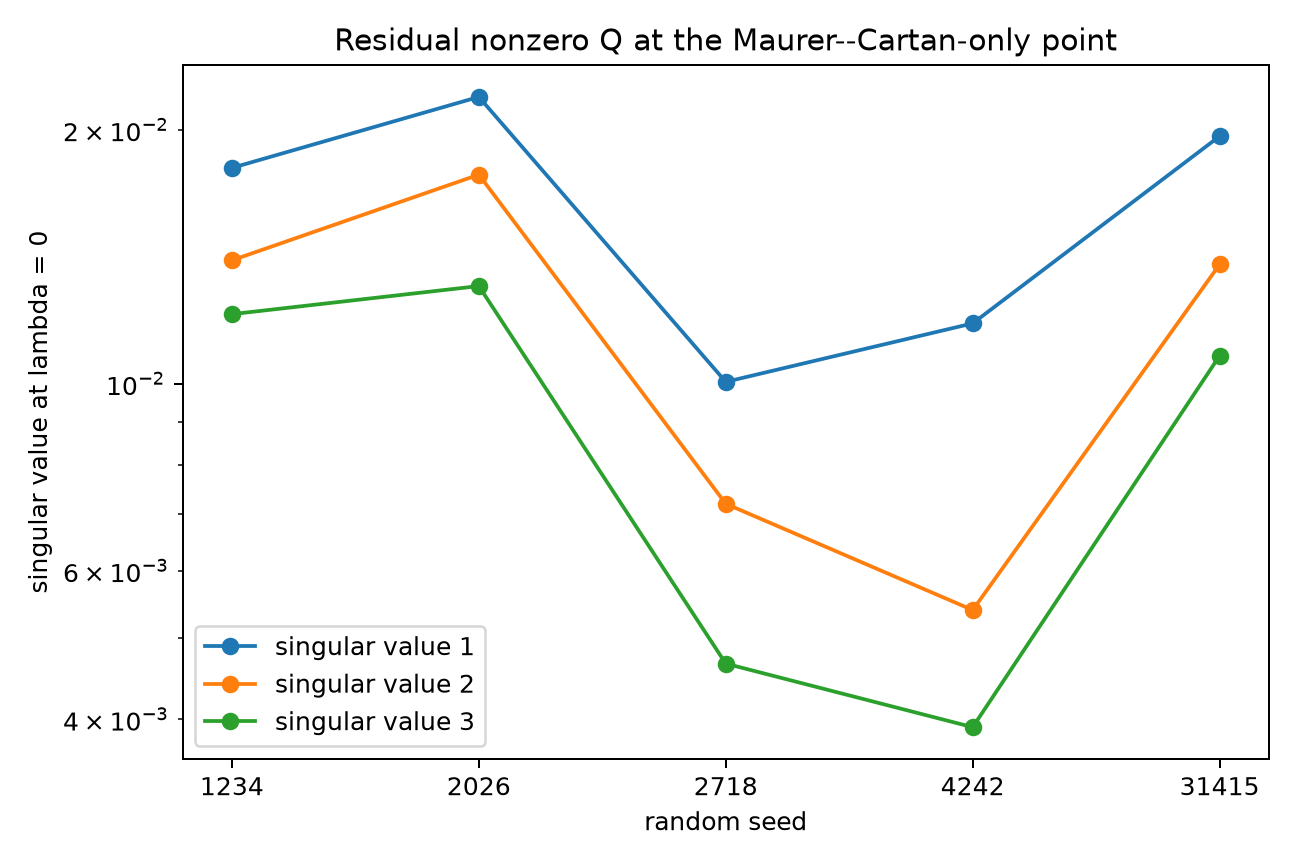
\includegraphics[width=0.82\linewidth]{../figures/01_pcm_fqe_multiseed/q_singular_values_lambda_zero_by_seed.png}
  \caption{$\lambda=0$ における learned $Q$ の singular values．解析解では三つともゼロであり，非零値は neural-network approximation error を表す．}
  \label{fig:pcm-q-zero-singular-values}
\end{figure}

この結果から，有限精度で学習した matrix に対して通常の numerical matrix rank をそのまま用いるのは適切でないことが分かる．厳密解でゼロの singular value も近似誤差によって非零になるからである．今後の dynamics-encoding diagnostic では，まず operator norm が通常の非零 scale に比べて抑制されているかを判定し，operator norm が十分に非零な点について singular-value ratios から rank loss を調べる．この二段階の診断を，flatness が equation of motion を encode しない既知の connection に適用する．

\section{今後の予定}

\subsection{共同研究者ノートの再現}

\subsubsection{Principal chiral model: bare flatness loss と再パラメータ化自由度の再現}
\subsubsection{Principal chiral model: analytic per-$\lambda$ reweighting の再現}
\subsubsection{Principal chiral model: component-norm normalization と adaptive weighting の再現}
\subsubsection{$S^2=SU(2)/U(1)$ sigma model: Jacobian null-space analysis の再現}
\subsubsection{$S^2=SU(2)/U(1)$ sigma model: pseudo-arclength continuation の再現}
\subsubsection{$S^2=SU(2)/U(1)$ sigma model: neural-network chart の再現}

\subsection{追加検証}

\subsubsection{$S^2=SU(2)/U(1)$ sigma model における off-shell factorization の学習}
\subsubsection{Flatness が equation of motion を encode しない既知の connection に対する singular-value diagnostic}
\subsubsection{複数のスペクトルパラメータで得た $Q(\lambda)$ を組み合わせた dynamics encoding の診断}
\subsubsection{Flatness solution manifold の tangent direction と Lax gauge orbit の分離}
\subsubsection{Spectral parameter の non-removability に対する数値診断}
\subsubsection{Jacobian null-space analysis, continuation, spectral charting の統一 pipeline}
\subsubsection{追加の既知可積分模型に対する benchmark}
\subsubsection{Learned Lax family からの monodromy と conserved quantities の検証}

\end{document}
